%Dokumentklasse

%draft als option ohne bilder für bessere performance
%\documentclass[a4paper,12pt,]{scrreprt}

%normal mit Bildern
\documentclass[
a4paper,
11pt,
draft=False]
{scrartcl}

%Section als Chapter
\RedeclareSectionCommand[%
%beforeskip = -1sp plus -1sp minus -1sp,% kleinster negativer Wert, um den Absatzeinzug nach der Überschrift zu verhindern.
afterskip = 1.5 \baselineskip plus -1sp minus 1sp,
font = \Huge,
]{section}

\usepackage[left= 3cm,right = 3cm, bottom = 3cm,top = 3cm]{geometry}
%\usepackage[onehalfspacing]{setspace}

% ============= Packages =============
% Dokumentinformationen
\usepackage[
pdftitle={Praktikum - Umwelttechnik},
pdfsubject={},
pdfauthor={Roman-Luca Zank},
pdfkeywords={},	
%Links nicht einrahmen
hidelinks
]{hyperref}

% Standard Packages
%\usepackage[bottom]{footmisc}
\usepackage[utf8]{inputenc}
\usepackage[ngerman]{babel}

\newcommand{\leadingzero}[1]{\ifnum #1<10 0\the#1\else\the#1\fi}
\newcommand{\todayDE}{\leadingzero{\day}.\leadingzero{\month}.\the\year} %dd.mm.yyyy
\usepackage[T1]{fontenc}
%\usepackage{helvet}

%\renewcommand{\familydefault}{\sfdefault}

\usepackage{graphicx}
\graphicspath{{img/}}
\usepackage[version=4]{mhchem}
\usepackage{fancyhdr}
	%\usepackage[automark]{scrlayer-scrpage}
	%\ihead{\leftmark}
	%\ohead*{\pagemark}
\usepackage{lmodern}
\usepackage{color}
\usepackage[bottom]{footmisc}
\usepackage{setspace}\usepackage{threeparttable}
%==================================================================
%\begin{threeparttable} 
%	\begin{tabular}{|l|c|r|} 
%		\hline 
%		A & B & C \\
%		\hline
%		1 & 2 & 3 \tnote{1} \\
%		\hline
%	\end{tabular} 
%	\begin{tablenotes}\footnotesize 
%		\item[1] Prognose 2003 
%	\end{tablenotes}
%====================================================================
\usepackage{placeins}
\usepackage{booktabs}
\usepackage{caption}
\usepackage[list=true]{subcaption}
\usepackage{longtable}
\usepackage{tikz}
\usepackage{pgfplots}
\pgfplotsset{compat=1.16}
\usepackage{lastpage}
%\usepackage{ulem}
\usepackage{mathtools}
\usepackage{adjustbox}
\usetikzlibrary{patterns}
\usepackage{pdfpages}

%Einheitenpackage
\usepackage{siunitx}  
\sisetup{	locale = DE, 
	per-mode=fraction,
	inter-unit-product=\ensuremath{\cdot},
	detect-weight = true,
	quotient-mode=fraction
}
%neue Einheiten definieren
\DeclareSIUnit\xyz{xyz}	
\DeclareSIUnit\rpm{rpm}	
\DeclareSIUnit\mws{mWS}	
\DeclareSIUnit\degrees{^\circ}	
\DeclareSIUnit\kmeter{\raiseto{3}\meter}	
\DeclareSIUnit\smeter{\raiseto{2}\meter}	
\DeclareSIUnit\g{\meter \per \raiseto{2}\second}	

%Automatisch cdot statt *
\DeclareMathSymbol{*}{\mathbin}{symbols}{"01}


%Tabelle
\usepackage{tabularx}
\usepackage{tabulary}

%nur letzte Zeile der Gleichung nummerieren
\makeatletter
\def\Let@{\def\\{\notag\math@cr}}
\makeatother

% zusätzliche Schriftzeichen der American Mathematical Society
\usepackage{amsfonts}
\usepackage{amsmath}

%Abkürzungsverzeichnis
\usepackage{acronym}

%kein Abstand bei neuem Kapitel vom Seitenanfang
%\vspace*{2.3\baselineskip} = ORIGINAL
%\renewcommand*{\chapterheadstartvskip}{\vspace*{.0\baselineskip}}

%nicht einrücken nach Absatz
\setlength{\parindent}{0pt}

\urlstyle{same}


% ============= Kopf- und Fußzeile =============
\pagestyle{fancy}
%
\lhead{}
\chead{}
\rhead{}%\slshape }%\leftmark}
%%
\lfoot{}
\cfoot{}
\rfoot[{\thepage\ of \pageref*{LastPage}}]{Seite \thepage\ von \pageref*{LastPage}}
%%
\renewcommand{\headrulewidth}{0pt}
\renewcommand{\footrulewidth}{0pt}
%\renewcommand{\chapterpagestyle}{fancy}

%Fußnotelinie
%\let\footnoterule

%Fußnote mit Klammer
\renewcommand*{\thefootnote}{(\arabic{footnote})}

%Abb. statt Abbildung
\addto\captionsngerman{%
	\renewcommand{\figurename}{Abb.}%
	\renewcommand{\tablename}{Tab.}%
}

% ============= Package Einstellungen & Sonstiges ============= 
%Besondere Trennungen
%\hyphenation{De-zi-mal-tren-nung}
\usepackage[none]{hyphenat}
\hyphenpenalty=5000
\tolerance=5000
\providecommand\phantomsection{}

\usepackage{mathtools}


% ============= Dokumentbeginn =============

\begin{document}
%Seiten ohne Kopf- und Fußzeile sowie Seitenzahl
\pagestyle{empty}

% Beendet eine Seite und erzwingt auf den nachfolgenden Seiten die Ausgabe aller Gleitobjekte (z.B. Abbildungen), die bislang definiert, aber noch nicht ausgegeben wurden. Dieser Befehl fügt, falls nötig, eine leere Seite ein, sodaß die nächste Seite nach den Gleitobjekten eine ungerade Seitennummer hat. 
\cleardoubleoddpage

% Pagestyle für Titelblatt leer
\pagestyle{empty}

%Seite zählen ab
\setcounter{page}{0}

%Titelblatt
\begin{center}
\begin{tabular}{p{\textwidth}}


\begin{center}

\includegraphics[scale=0.75]{logos.jpg}\\
\end{center}


\\

\begin{center}
\LARGE{\textsc{Einführung in die Laborpraktika\\
}}
\end{center}

\\

%\begin{center}
%\large{Fakultät für Muster und Beispiele \\
%der Hochschule Musterhausen \\}
%\end{center}
%
%\\

\begin{center}
\textbf{\Large{Handout mit allgemeinen Hinweisen für \mbox{chemie- und umwelttechnische} Praktika}}
\end{center}


\\
%\begin{center}
%zur Erlangung des akademischen Grades\\
%Bachelor of Engineering
%\end{center}


%\begin{center}
%vorgelegt von
%\end{center}

\begin{center}
	\includegraphics[scale=0.75]{img/versuchsaufbau_1}\\
\end{center}
%Ende

\begin{center}
	Diese Übersicht soll für zukünftige Praktika in Form von Vorschlägen und Wissen eine Unterstützung bieten, um Geräte oder Versuchsstände selbstständig bedienen und aufbauen zu können.
\end{center}


\\ \\

%\begin{center}
%\begin{tabular}{lll}
%\large{\textbf{Protokollführer:}} & & \large{Roman-Luca Zank}\\
%&&\\
%\large{\textbf{Datum der Versuchsdurchführung:}}&& \large{22.10.2020}\\
%&&\\
%\large{\textbf{Abgabedatum:}}&& \large{\todayDE}
%\end{tabular}
%\end{center}

\end{tabular}
\end{center}

\vfill
\large{Merseburg den \todayDE}
 %Prokolle
%\begin{center}
\begin{tabular}{p{\textwidth}}


\begin{center}

\includegraphics[scale=0.75]{img/logos.jpg}\\
\end{center}


\\

\begin{center}
\LARGE{\textsc{
Recherche \\
Rückgewinnung von Ammoniak aus Industrieabwässern\\
}}
\end{center}

%\begin{center}
%\large{Fakultät für Muster und Beispiele \\
%der Hochschule Musterhausen \\}
%\end{center}
%
%\\
 \\
 
\begin{center}
\textbf{\Large{Seminararbeit in Medienrecherche}}
\end{center}

\begin{center}
	\large{im WiSe 2019}
\end{center}
 \\
%\begin{center}
%zur Erlangung des akademischen Grades\\
%Bachelor of Engineering
%\end{center}


\begin{center}
\large{vorgelegt von}
\end{center}
\\


\begin{center}
\Large{\textbf{Roman-Luca Zank}} \\
\end{center}

\begin{center}
3. Semester \\
Chemie- und Umwelttechnik \\
\end{center}


\begin{center}
\begin{tabular}{lll}
	\textbf{E-Mail:} & & romanzank@mail.de\\
	\textbf{Matrikelnummer:} & &25240\\
	\textbf{Adresse:} & &Platz der Bausoldaten 2, Zimmer 224\\
	\textbf{Ort:} & &06217 Merseburg\\
	&& \\
	\textbf{Prüfer:} & & Dr. Frank  Baumann\\
\end{tabular}
\end{center}

\\ \\ \\ \\ \\
\large{Merseburg, \today}

\end{tabular}
\end{center}
 %Seminar-/Abschlussarbeit

% Pagestyle für Rest des Dokuments
\pagestyle{fancy}

%Inhaltsverzeichnis
\tableofcontents
\thispagestyle{empty}

%Inhalt
%
%Verzeichnis aller Bilder
\label{sec:bilder}
\listoffigures
\addcontentsline{toc}{chapter}{Abbildungsverzeichnis}
\thispagestyle{empty}

%Verzeichnis aller Tabellen
\label{sec:tabellen}
\listoftables
\addcontentsline{toc}{chapter}{Tabellenverzeichnis}
\thispagestyle{empty}



%\include{0A_abkurzungsverzeichnis}
\section{Übung 1}
\subsection*{a$)$}

\begin{minipage}[t]{0.33\textwidth}
$\underline{\text{Gegeben:}}$
\begin{itemize}
	\item V=70 \si{\liter}
	\item p=2 \si{\bar}
	\item $\text{p}_0$=1000 \si{\hecto\pascal}
	\item T=(20+273)\si{\kelvin}=293\si{\kelvin}
\end{itemize}
\end{minipage}
\begin{minipage}[t]{0.33\textwidth}
	$\underline{\text{Gesucht:}}$
	\begin{itemize}
		\item $\rho$
		\item m$_{Luft}$
	\end{itemize}
\end{minipage}
\begin{minipage}[t]{0.33\textwidth}
	$\underline{\text{Verwendete Formeln:}}$
	\begin{equation}
	p*V=n*R*T
	\end{equation}
	\begin{equation}
	\rho =\frac{m}{V}
	\end{equation}
	\begin{equation}
	\text{p}_{abs} =\text{p}+\text{p}_0
	\end{equation}
\end{minipage}

\vspace{1cm}

Der Reifendruckmesser (Manometer) zeigt den Überdruck gegenüber der Atmosphäre an.

\begin{equation}
p_0=\SI{1000}{\hecto\pascal}=\underline{10^5 \si{\pascal}}=\SI{1}{\bar}
\end{equation}
\begin{equation}
	\text{p}_{abs}=10^5\si{\pascal}+2*10^5\si{\pascal}=\underline{3*10^5\si{\pascal}}
\end{equation}
\begin{flalign}
p*V&=n*R*T\\
&=m*R_i*T\\
p&=\frac{m}{V}*R_i*T\\
\rho=\frac{m}{V}&=\frac{p_{abs}}{R_i*T}
\end{flalign}
\begin{flalign}
	\rho&=\frac{3*10^5\si{\pascal}}{\SI{287,6}{\joule\per\kilogram\per\kelvin}*\SI{293}{\kelvin}}\\
	&=\underline{\underline{\SI{3,565}{\kilogram\per\cubic\meter}}}
\end{flalign}
\begin{flalign}
	m&=\rho*V\\
	&=\SI{3,565}{\kilogram\per\cubic\meter}*\SI{0,07}{\cubic\meter}\\
	&=\underline{\underline{\SI{0,25}{\kilogram}}}
\end{flalign}





\subsection*{b$)$}
\begin{minipage}[t]{0.33\textwidth}
	$\underline{\text{Gegeben:}}$
	\begin{itemize}
		\item 
		\item 
		\item 
		\item 
	\end{itemize}
\end{minipage}
\begin{minipage}[t]{0.33\textwidth}
	$\underline{\text{Gesucht:}}$
	\begin{itemize}
		\item 
		\item 
	\end{itemize}
\end{minipage}
\begin{minipage}[t]{0.33\textwidth}
	$\underline{\text{Verwendete Formeln:}}$
	\begin{equation}
	
	\end{equation}
	\begin{equation}
	
	\end{equation}
	\begin{equation}
	
	\end{equation}
\end{minipage}


\subsection*{c$)$}
\begin{minipage}[t]{0.33\textwidth}
	$\underline{\text{Gegeben:}}$
	\begin{itemize}
		\item 
		\item 
		\item 
		\item 
	\end{itemize}
\end{minipage}
\begin{minipage}[t]{0.33\textwidth}
	$\underline{\text{Gesucht:}}$
	\begin{itemize}
		\item 
		\item 
	\end{itemize}
\end{minipage}
\begin{minipage}[t]{0.33\textwidth}
	$\underline{\text{Verwendete Formeln:}}$
	\begin{equation}
	
	\end{equation}
	\begin{equation}
	
	\end{equation}
	\begin{equation}
	
	\end{equation}
\end{minipage}



\setcounter{equation}{0}
\section{Übung 2}
\subsection*{a$)$}

\begin{minipage}[t]{0.33\textwidth}
$\underline{\text{Gegeben:}}$
\begin{itemize}
	\item $F_{Hand}=\SI{100}{\newton}$
	\item $d_1=\SI{0,015}{\meter}$
	\item $d_2=\SI{0,05}{\meter}$
	\item $l_1=\SI{0,33}{\meter}$
	\item $l_2=\SI{0,03}{\meter}$
\end{itemize}
\end{minipage}
\begin{minipage}[t]{0.33\textwidth}
	$\underline{\text{Gesucht:}}$
	\begin{itemize}
		\item Übersetzungsverhältnis gesamt $\frac{F_2}{F_{Hand}}$
		\item Übersetzung hydrau\-lische Seite
	\end{itemize}
\end{minipage}
\begin{minipage}[t]{0.33\textwidth}
	$\underline{\text{Verwendete Formeln:}}$
	\begin{equation}
	\frac{F_1}{F_2}=\frac{A_2}{A_1}=\frac{l_2}{l_1}
	\end{equation}
\end{minipage}

\vspace{1cm}

Beachte, es liegt ein einseitiger Hebel vor! Darum besteht der lange Hebelarm $l_1$ aus dem gesamten Hebel, und nicht nur aus einer Seite vom Gelenk aus.
\begin{flalign}
A1&= \frac{\pi}{4}*d_1^2= \frac{\pi}{4}*(\SI{0,015}{\meter})^2\\
&= \underline{\SI{176,5e-6}{\smeter}}\\
A2&= \frac{\pi}{4}*d_2^2= \frac{\pi}{4}*(\SI{0,05}{\meter})^2\\
&= \underline{\SI{1962,5e-6}{\smeter}}
\end{flalign}

Wirkung des Hebels:
\begin{flalign}
	\frac{F_{Hand}}{F1}&=\frac{l_1}{l_2}\\
	F_1&=F_{Hand}*\frac{l_1}{l_2}=\SI{100}{\newton}*\frac{\SI{0,33}{\meter}}{\SI{0,03}{\meter}}\\
	&=\underline{\SI{1100}{\newton}}
\end{flalign}
Wirkung der Hydraulik:
\begin{flalign}
	\frac{F_1}{F_2}&=\frac{A_2}{A_1}\\
	F_2&=F_1*\frac{A_2}{A_1}\\
	&=\SI{1100}{\newton}*\frac{\SI{1962,5e-6}{\smeter}}{\SI{176,5e-6}{\smeter}}\\
	&=\underline{\SI{12230,9}{\newton}}
\end{flalign}
\begin{flalign}
	\frac{F_{2}}{F_{Hand}}&=\frac{\SI{12230,9}{\newton}}{\SI{100}{\newton}}=\underline{\underline{122,309}}
\end{flalign}
\begin{flalign}
\frac{F_{2}}{F_{1}}&=\frac{\SI{12230,9}{\newton}}{\SI{1100}{\newton}}=\underline{\underline{11,119}}
\end{flalign}


\subsection*{b$)$ - normal}

\begin{minipage}[t]{0.33\textwidth}
	$\underline{\text{Gegeben:}}$
	\begin{itemize}
		\item $F=\SI{200}{\newton}$
		\item $d_1=\SI{0,03}{\meter}$
		\item $d_2=\SI{0,02}{\meter}$
		\item $l_1=\SI{0,35}{\meter}$
		\item $l_2=\SI{0,07}{\meter}$
	\end{itemize}
\end{minipage}
\begin{minipage}[t]{0.33\textwidth}
	$\underline{\text{Gesucht:}}$
	\begin{itemize}
		\item Systemdruck $p$
		\item Anpressdruck der Bremsbacken $F_2$
	\end{itemize}
\end{minipage}
\begin{minipage}[t]{0.33\textwidth}
	$\underline{\text{Verwendete Formeln:}}$
	\begin{equation}
	\frac{F_1}{F_2}=\frac{A_2}{A_1}=\frac{l_2}{l_1}
	\end{equation}
	\begin{equation}
		p=\frac{F}{A}
	\end{equation}
\end{minipage}

\vspace{1cm}

Wirkung des Hebels:
\begin{flalign}
\frac{F}{F_1}&=\frac{l_1}{l_2}\\
F_1&=F*\frac{l_1}{l_2}=\SI{200}{\newton}*\frac{\SI{0,35}{\meter}}{\SI{0,07}{\meter}}\\
&=\underline{\SI{1000}{\newton}}
\end{flalign}


Druck im System:

Druck ist Kraft pro Fläche.

\begin{flalign}
	p_1&=\frac{F1}{A1}\\
	&=\frac{\SI{1000}{\newton}}{\frac{\pi}{4}*(\SI{0,03}{\meter})^2}\\
	&=\underline{\underline{\SI{1,415E6}{\pascal}}}
\end{flalign}

Druck auf die Bremsbacken:

\begin{flalign}
F&=A*p\\
F_2&=A_2*p_1=\left( \frac{\pi}{4}*(\SI{0,02}{\meter})^2 \right) *\SI{1,415E6}{\pascal}\\
&= \underline{\underline{\SI{444,5}{\newton}}}
\end{flalign}



\newpage

\subsection*{b$)$ - Druckwandler}

\begin{minipage}[t]{0.33\textwidth}
	$\underline{\text{Gegeben:}}$
	\begin{itemize}
		\item $d_1=\SI{0,016}{\meter}$
		\item $d_{1,2}=\SI{0,04}{\meter}$
		\item $d_2= \SI{0,018}{meter}$
		\item $l_1=\SI{0,35}{\meter}$
		\item $l_2=\SI{0,07}{\meter}$
	\end{itemize}
\end{minipage}
\begin{minipage}[t]{0.33\textwidth}
	$\underline{\text{Gesucht:}}$
	\begin{itemize}
		\item Benötigte Kraft am Bremspedal ($F_{neu}$)
		
	\end{itemize}
\end{minipage}
\begin{minipage}[t]{0.33\textwidth}
	$\underline{\text{Verwendete Formeln:}}$
	\begin{equation}
	\frac{F_1}{F_2}=\frac{A_2}{A_1}=\frac{l_2}{l_1}
	\end{equation}
	\begin{equation}
		\frac{p_1}{p_2}=\frac{A_2}{A_1}=\frac{d_2}{d_1}
	\end{equation}
\end{minipage}

\vspace{1cm}

\begin{flalign}
	\frac{F_{neu}}{F_1}&=\frac{l_2}{l_1}\\
	F_1&=p_2*A_2\\
	p_2&=\frac{d_1^2*p_1}{d_{1,2}^2}
\end{flalign}
Zusammengesetzt:
\begin{equation}
	\frac{l_2}{l_1}=\frac{F_{neu}}{\left( \frac{d_1^2*p_1}{d_{1,2}^2} \right)  *A_2}
\end{equation}
\begin{flalign}
F_{neu}&=\frac{A_2*d_1^2*p_1*l_2}{d_{1,2}^2*l_1}\\
&=\frac{(\frac{\pi}{4}*(d_2)^2)*d_1^2*p_1*l_2}{d_{1,2}^2*l_1}\\
&=\frac{(\frac{\pi}{4}*(\SI{0,018}{meter})^2)*(\SI{0,016}{\meter})^2*\SI{1,415E6}{\pascal}*\SI{0,07}{\meter}}{(\SI{0,04}{\meter})^2*\SI{0,35}{\meter}}\\
&=\underline{\underline{\SI{11,52}{\newton}}}
\end{flalign}
\setcounter{equation}{0}
\section{Übung 13}
\begin{minipage}[t]{0.33\textwidth}
	$\underline{\text{Gegeben:}}$
	\begin{itemize}
		\item $H = \SI{3}{\meter}$
		\item $R = \SI{200}{\milli \meter} = \SI{0,2}{\meter}$
		\item $T_{\ce{H2O}}= \SI{20}{\celsius}$
	\end{itemize}
\end{minipage}
\begin{minipage}[t]{0.33\textwidth}
	$\underline{\text{Gesucht:}}$
	\begin{itemize}
		\item $\overrightarrow{F}_{\text{res}}$
	\end{itemize}
\end{minipage}
\begin{minipage}[t]{0.33\textwidth}
	$\underline{\text{Verwendete Formeln:}}$
		\begin{equation}
			p = \rho*g*h
		\end{equation}
		\begin{align}
			\overrightarrow{F} &= A*p \\
			&= \rho*g*V
		\end{align}
		\begin{equation}
			A = \pi * r^2
			\end{equation}
\end{minipage}

\textit{Zur Erinnerung: }
\begin{flalign*}
	\left[ \si{\kg \per \kmeter}*\si{\per\raiseto{2} \second} = \si{\newton \per \smeter} = \si{\pascal}\right]\\
\end{flalign*}

\begin{flalign}
	\text{\textbf{Annahme}: Da } T_{\ce{H2O} }= \SI{20}{\celsius} \text{ ist, ist } \rho_{\ce{H2O}} = \SI{1000}{\kg \per \kmeter}
\end{flalign}

\begin{figure}[h!]
	\centering
	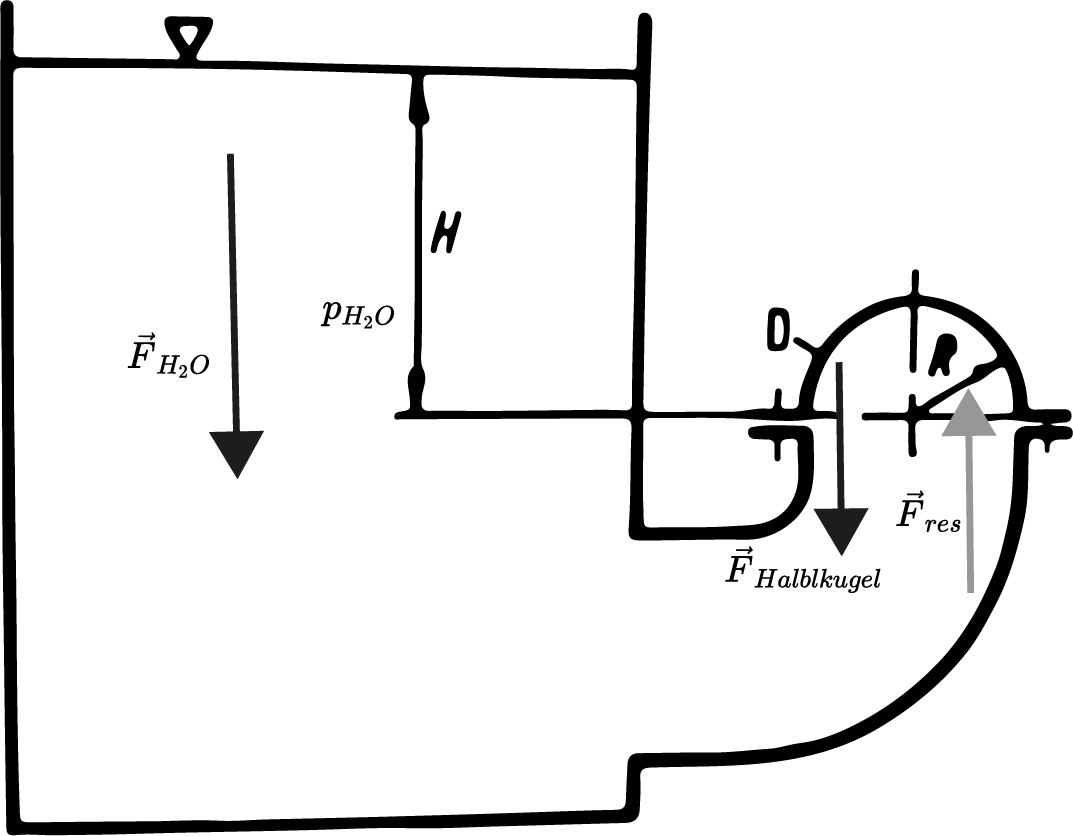
\includegraphics[width=0.4\textwidth]{u13}
\end{figure}
\FloatBarrier
%Ende

\begin{flalign}
	p_{\ce{H2O}} &= \rho_{\ce{H2O}}*g*h\\
								&= \SI{1000}{\kg \per \kmeter}*\SI{9,81}{\meter \per \raiseto{2} \second}*\SI{3}{\meter}\\
								&= \underline{\SI{29430}{\pascal}}
\end{flalign}
\begin{flalign}
	A_{\text{Halbkugel}} &= R^2*\pi\\
	&= \SI{0,2}{\meter}^2*\pi\\
	&= \underline{\SI{0,126}{\smeter}}
\end{flalign}
\begin{flalign}
	\overrightarrow{F}_{\text{\ce{H2O}}} &=A_{\text{Halblkugel}}*p_{\ce{H2O}}\\
	&= \SI{0,126}{\smeter}*\SI{29430}{\newton \per \smeter}\\
	&= \underline{\SI{3698,3}{\newton}}
\end{flalign}
\begin{flalign}
	\overrightarrow{F}_{\text{Halblkugel}} &=\rho_{\ce{H2O}}*g*V_{\text{Halbkugel}}\\
		&= \SI{1000}{\kg\per\kmeter}*\SI{9,81}{\meter \per \raiseto{2}\second}*\frac{1}{2}*\frac{4}{3}*\pi*\SI{0,2}{\smeter}^3\\
		&= \underline{\SI{164,4}{\newton}}
\end{flalign}
\begin{flalign}
	\overrightarrow{F}_{\text{res}} &=\overrightarrow{F}_{\ce{H2O}}-\overrightarrow{F}_{\text{Halblkugel}} \\
			&= \SI{3698,3}{\newton}-\SI{164,4}{\newton}\\
			&= \underline{\underline{\SI{3533,9}{\newton}}}
\end{flalign}

\setcounter{equation}{0}
\section{Übung 108}
\begin{minipage}[t]{0.33\textwidth}
	$\underline{\text{Gegeben:}}$
	\begin{itemize}
		\item $h = \SI{30}{\centi \meter}= \SI{0,3}{\meter}$
		\item  $m_{\text{OK}} = \SI{485}{\kg}$
		\item $\rho_{GG} = \SI{7,2}{\kg \per \liter}=\SI{7200}{\kg \per \kmeter}$
		\item $D = \SI{825}{\milli \meter} = \SI{0,825}{\meter}$
		\item $d = \SI{270}{\milli \meter} = \SI{0,270}{\meter}$
		\item $s = \SI{100}{\milli \meter} = \SI{0,1}{\meter}$
	\end{itemize}
\end{minipage}
\begin{minipage}[t]{0.33\textwidth}
	$\underline{\text{Gesucht:}}$
	\begin{itemize}
		\item $\overrightarrow{F}_{\text{Schraube}}$
	\end{itemize}
\end{minipage}
\begin{minipage}[t]{0.33\textwidth}
	$\underline{\text{Verwendete Formeln:}}$
		\begin{align}
			\overrightarrow{F} &= m*g \\
			&= \rho*g*A*h
		\end{align}
		\begin{equation}
			A = \frac{\pi}{4}*\left(D^2-d^2\right)
			\end{equation}
\end{minipage}

\vspace*{5mm}

\textit{Zur Erinnerung: }
\begin{flalign*}
	\overrightarrow{F}_{\text{Auftrieb}} &= V*g*\rho
\end{flalign*}

\begin{figure}[h!]
	\centering
	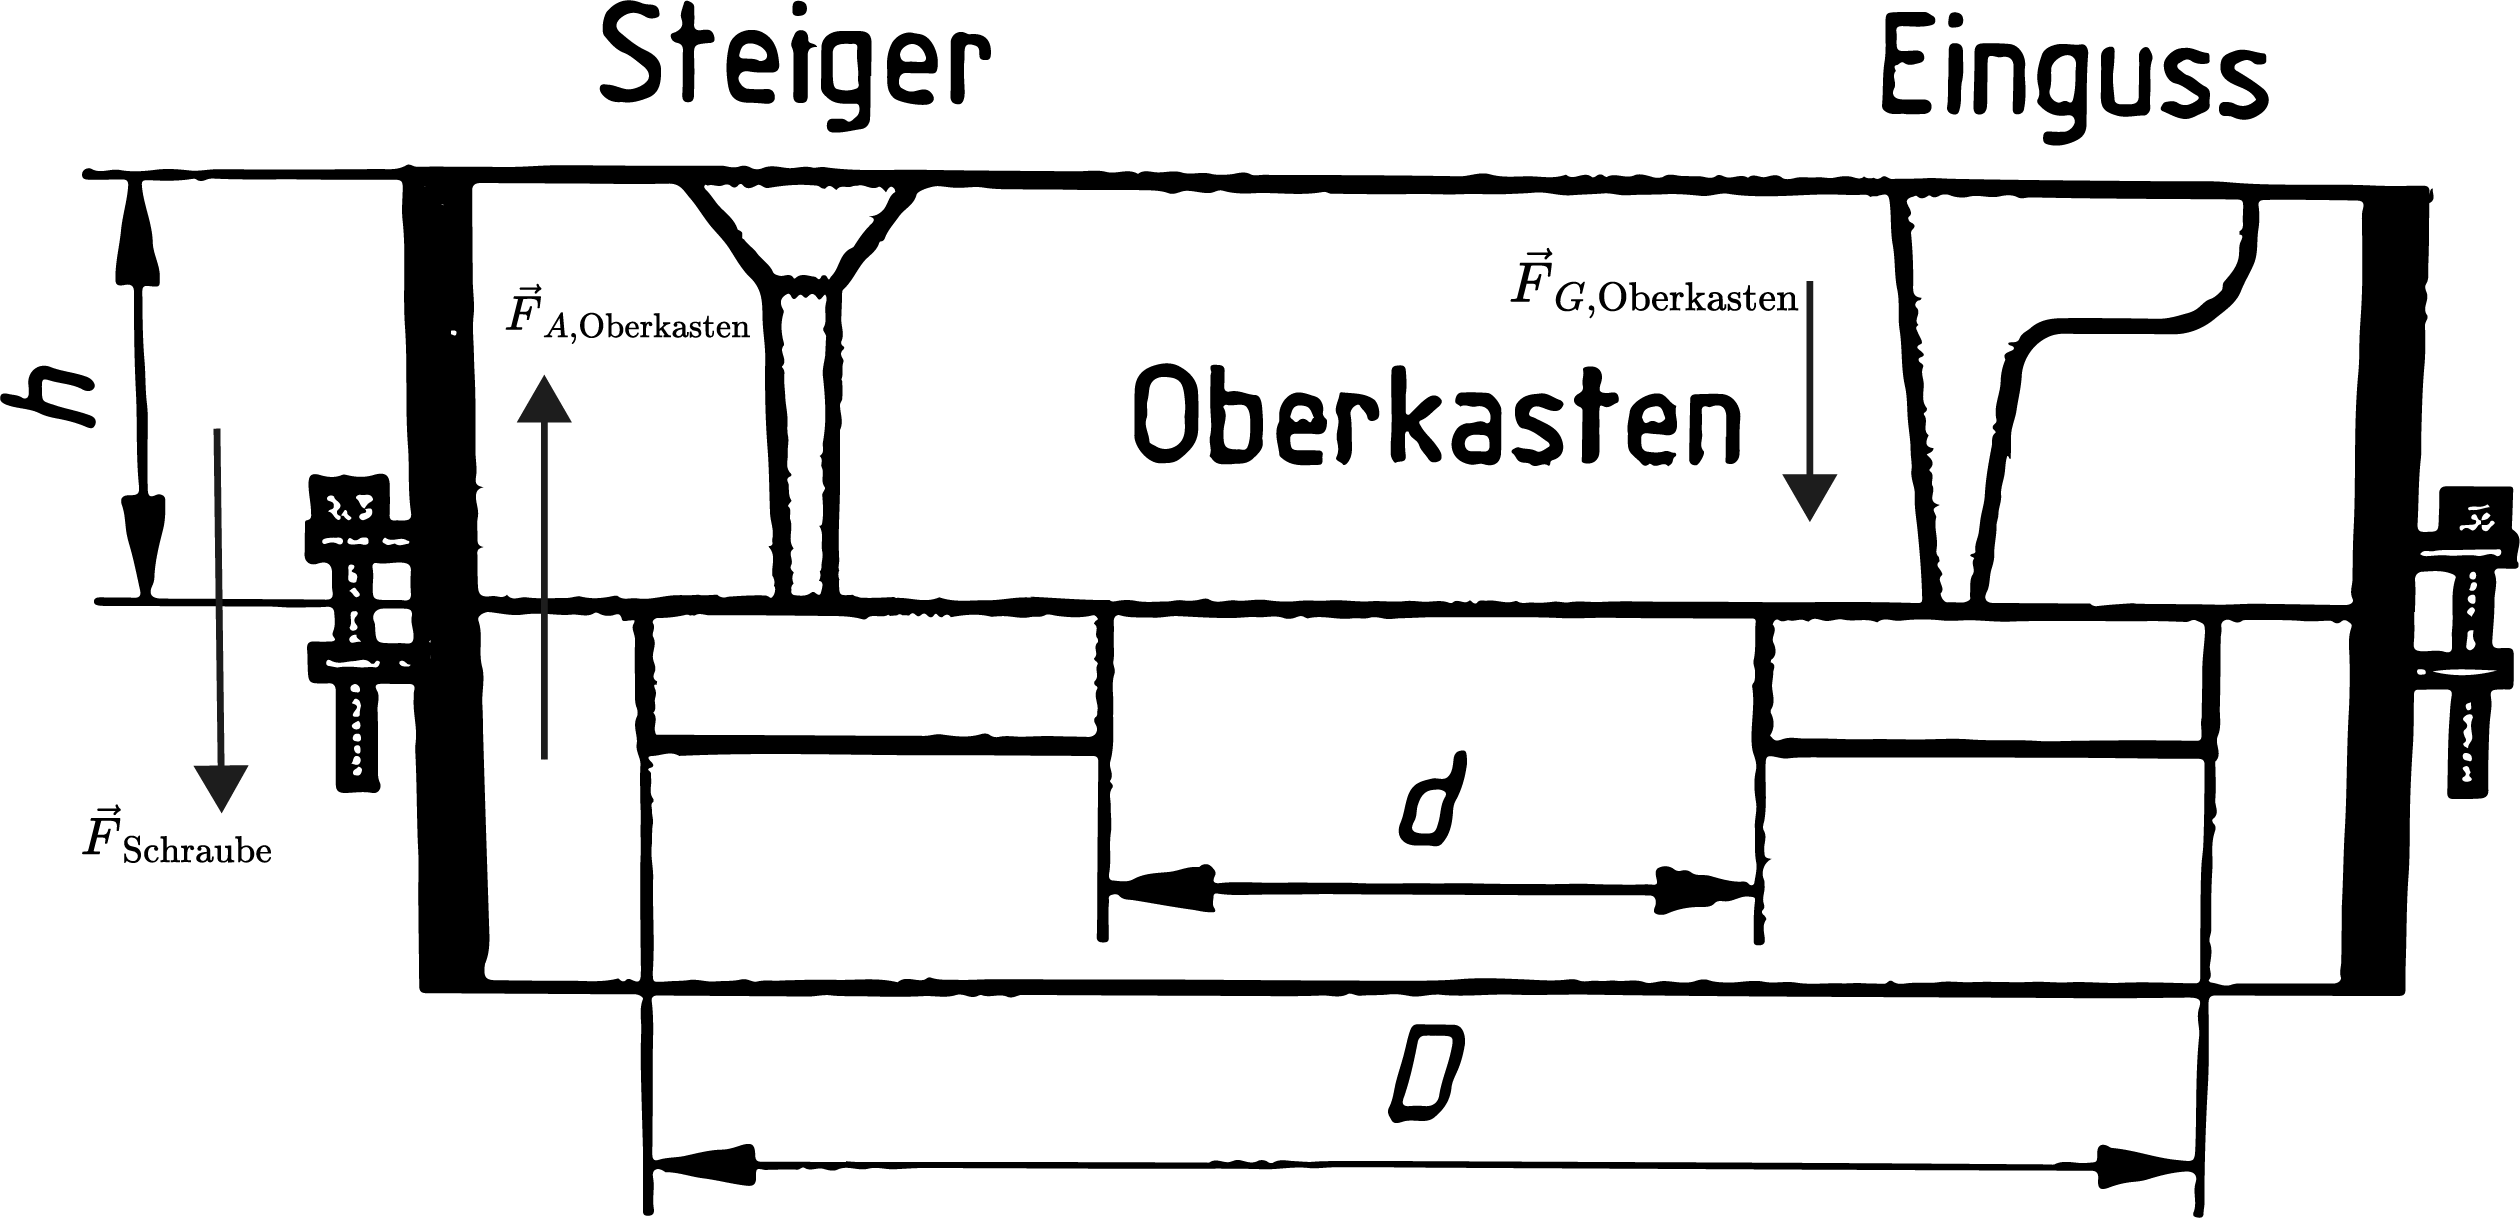
\includegraphics[width=0.8\textwidth]{u108}
\end{figure}
\FloatBarrier
%Ende

\begin{flalign}
	\overrightarrow{F}_{G, \text{Oberkasten}} &= m*g\\
	&= \SI{485}{\kg}*\SI{9,81}{\g}\\
	&= \underline{\SI{4747,85}{\newton}}
\end{flalign}
\begin{flalign}
	A_{\text{proj}}&= \frac{\pi}{4}*\left(D^2-d^2\right)\\
	&= \frac{\pi}{4}*\left(\SI{0,825}{\meter}^2-\SI{0,270}{\meter^2}\right)\\
	&= \underline{\SI{0,477}{\smeter}}
\end{flalign}
\begin{flalign}
	\overrightarrow{F}_{A, \text{Oberkasten}} &= A_{\text{proj}}*\rho_{GG}*g*h\\
	&= \SI{0,477}{\smeter}*\SI{7200}{\kg\per \kmeter}*\SI{9,81}{\g}*\SI{0,3}{\meter}\\
	&= \underline{\SI{10107,4}{\newton}}
\end{flalign}
\begin{flalign}
	\overrightarrow{F}_{A, \text{Oberkasten}} &= A_{\text{proj}}*\rho_{GG}*g*h\\
	&= \SI{0,477}{\smeter}*\SI{7200}{\kg\per \kmeter}*\SI{9,81}{\g}*\SI{0,3}{\meter}\\
	&= \underline{\SI{10107,4}{\newton}}
\end{flalign}
\begin{flalign}
	\overrightarrow{F}_{\text{Schraube}} &= 
	\overrightarrow{F}_{A, \text{Oberkasten}} -\overrightarrow{F}_{G, \text{Oberkasten}} \\
	&= \underline{\underline{\SI{5359,6}{\newton}=\SI{5,36}{\kilo \newton}}}
\end{flalign}



%\section*{Anhang}
\addcontentsline{toc}{section}{Anhang}
\label{sec:anhang}

%Betriebsanweisung
%%Praktikumsskript, Modul ………, Versuch …….., Prof. Musterprof. 
%DIN 12345, Jahr der Veröffentlichung 
%Link der Internetseite, Zugriffsdatum 
%Buchtitel, Autor, Verlag, Veröffentlichungsjahr 

%Literaturverzeichnis Bücher
\bibliography{Literatur}
\bibliographystyle{unsrtdin}
\addcontentsline{toc}{section}{Literaturverzeichnis}





\end{document}
